\documentclass[tikz,border=8pt]{standalone}
\usepackage{amsmath}
\usetikzlibrary{arrows.meta,positioning,shapes.geometric}
\begin{document}
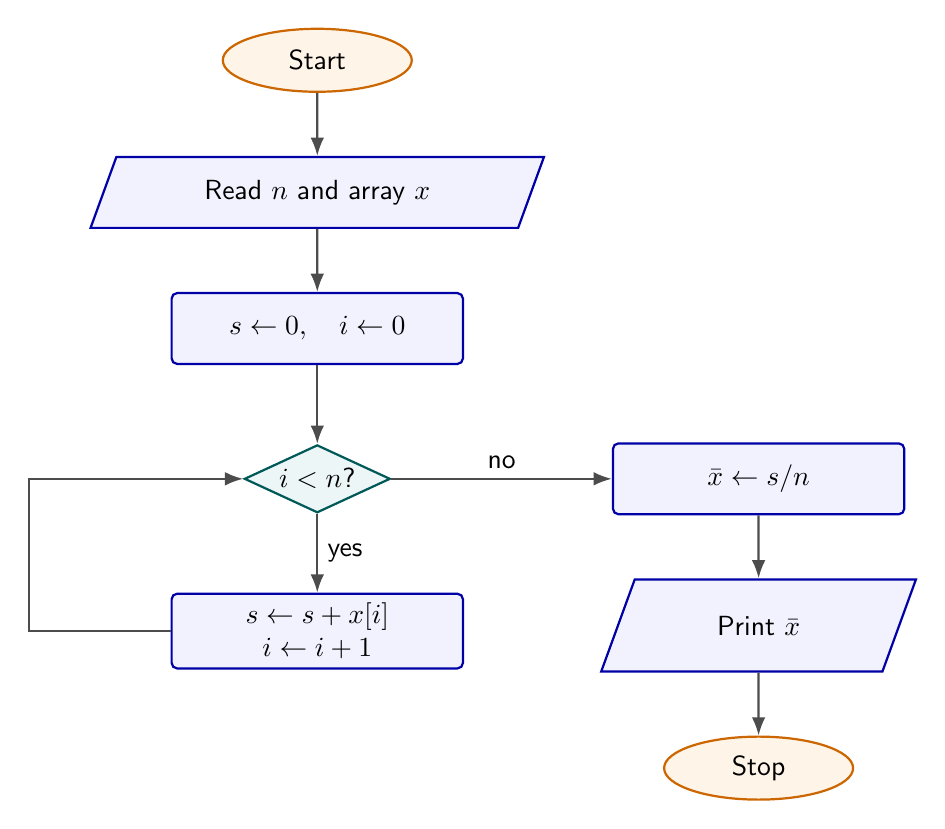
\begin{tikzpicture}[
  >=Latex,
  font=\sffamily,
  node distance=8mm and 18mm,
  flow/.style={draw=blue!65!black,thick,rounded corners=2pt,fill=blue!5,
    minimum width=37mm,minimum height=9mm,align=center},
  io/.style={trapezium,trapezium left angle=70,trapezium right angle=110,
    draw=blue!65!black,thick,fill=blue!5,
    minimum width=40mm,minimum height=9mm,align=center},
  decision/.style={diamond,draw=teal!70!black,thick,fill=teal!7,
    aspect=2.15,inner sep=1.5pt,align=center},
  terminal/.style={ellipse,draw=orange!80!black,thick,fill=orange!9,
    minimum width=24mm,minimum height=8mm,align=center},
  line/.style={->,thick,draw=black!70}
]
  \node[terminal] (start) {Start};
  \node[io,below=of start] (read) {Read $n$ and array $x$};
  \node[flow,below=of read] (init) {$s\gets0,\quad i\gets0$};
  \node[decision,below=10mm of init] (test) {$i<n$?};
  \node[flow,below=10mm of test] (update) {$s\gets s+x[i]$\\$i\gets i+1$};
  \node[flow,right=28mm of test] (mean) {$\bar{x}\gets s/n$};
  \node[io,below=of mean] (print) {Print $\bar{x}$};
  \node[terminal,below=of print] (stop) {Stop};

  \draw[line] (start)--(read);
  \draw[line] (read)--(init);
  \draw[line] (init)--(test);
  \draw[line] (test)--node[right]{yes}(update);
  \draw[line] (update.west)-| ++(-18mm,0) |- (test.west);
  \draw[line] (test)--node[above]{no}(mean);
  \draw[line] (mean)--(print);
  \draw[line] (print)--(stop);
\end{tikzpicture}
\end{document}
